\documentclass[11pt]{scrartcl}
\usepackage{graphicx}
\graphicspath{{./}}
\usepackage[sexy]{evan}
\usepackage[normalem]{ulem}
\usepackage{hyperref}
\usepackage{mathtools}
\hypersetup{
    colorlinks=true,
    linkcolor=blue,
    filecolor=magenta,      
    urlcolor=cyan,
    pdfpagemode=FullScreen,
    }

\renewcommand{\baselinestretch}{1.5}

\addtolength{\oddsidemargin}{-0.4in}
\addtolength{\evensidemargin}{-0.4in}
\addtolength{\textwidth}{0.8in}

\setlength{\parindent}{0pt}

\usepackage{pgfplots}
\pgfplotsset{compat=1.15}
\usepackage{mathrsfs}
\usetikzlibrary{arrows}

\begin{document}
	\title{Post Test} % Beginner
	\date{}
	\author{Pelatihan KSN-K}
	\maketitle
	
	Aturan Umum
	\begin{itemize}
	    \item Ujian ini tediri dari 16 soal isian singkat.
	    \item Poin maksimum yang mungkin didapat pada ujian ini adalah 100 poin.
	    \item Setiap soal dipastikan memiliki solusi berupa bilangan bulat non-negatif.
	    \item Setiap soal memiliki poin bervariasi sesuai keterangan di sebelah nomor soal jika dijawab benar.
	    \item Setiap soal yang dijawab salah atau kosong bernilai 0.
	\end{itemize}
	
	\section{Soal}
	\begin{enumerate}
	    \item (3 poin) Pada $\triangle ABC$ terdapat titik $D$ pada segmen $BC$ sehingga $BD:DC=1:3$. Titik $L$ pada $AD$ sehingga $AL:LD=1:4$. Jika $\dfrac{[ACL]}{[BDL]}=k$, tentukan nilai $200k$.
	    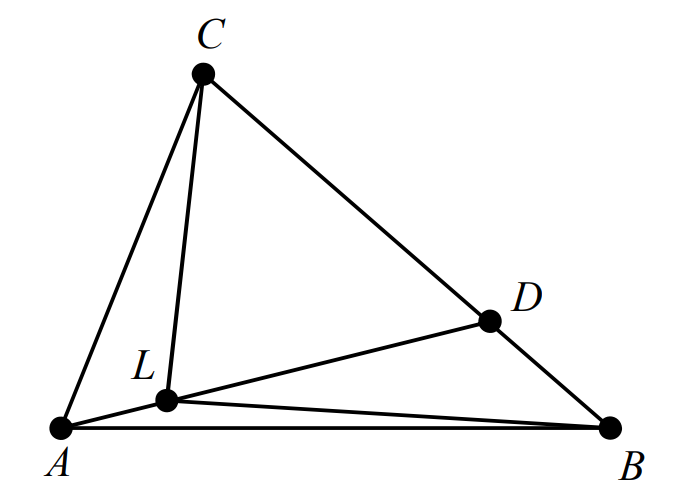
\includegraphics[scale=0.5]{geogampang.PNG}
	    
	    \item (3 poin) Misalkan suatu fungsi $f:\RR \rightarrow \RR$ memenuhi $f(xy)=f(x+y)$ untuk seluruh bilangan real $x$ dan $y$. Jika $f(-10)=10$ berapakah nilai $2021\cdot f(2021)$?
	    
	    \item (3 poin) Banyak bilangan asli yang kurang dari 10000 dengan jumlah digit pertama dan digit terakhirnya sama dengan 11 adalah \dots
	    
	    \item (3 poin) Jika diketahui bahwa $x=\dfrac{3^{15}-1}{2}$ adalah bilangan asli, maka sisa saat $x$ dibagi $9$ adalah \dots
	    
	    
	    \item (5 poin) Misalkan $x,y,z$ adalah bilangan real yang memenuhi $2^x=3^y=6^z.$
	    
	    Nilai $116+\dfrac{1}{x}+\dfrac{1}{y}-\dfrac{1}{z}=\dots$
	    
	    \item (5 poin) Diketahui bahwa ketiga bilangan $p$, $p+8$, dan $p+16$ adalah bilangan prima. Tentukan jumlah semua nilai $p$ yang mungkin.
	    
	    \item (5 poin) Wadah pertama berisi 5 kelereng merah dan 4 kelereng biru. Wadah kedua berisi 7 kelereng merah dan
		9 kelereng biru. Sebuah kelereng dipindahkan dari wadah pertama ke wadah kedua. Selanjutnya, sebuah
		kelereng diambil dari wadah kedua, jika peluang yang terambil bola merah adalah
		$\frac{a}{b}$. Tentukan nilai dari $a+b$ dimana $a, b$ bilangan bulat positif yang saling prima.
	    
	    \item (5 poin) Diberikan sebuah trapesium siku-siku $ABCD$ dimana $BC$ tegak lurus $CD$ dengan $AB$ sejajar $CD$ dan $AB < CD$. jika panjang $AB = 1$, $BD = \sqrt{7}$, dan $AD = CD$, Jika luas trapesium tersebut adalah $S$, maka nilai $4S^2$ adalah \dots
	    
	    \item (7 poin) Banyaknya pasangan terurut bilangan asli $(m,n)$ yang memenuhi $$m^3+n^3=(m+n)^2$$ adalah \dots
	    
	    \item (7 poin) Ekspresi $$x^2+\left(\dfrac{x}{2x-1}\right)^2=2$$ mempunyai tiga solusi real $x$. Tentukan jumlah seluruh solusi real $x$ tersebut.
	    % https://www.youtube.com/watch?v=E2s7cMERjJo&list=WL&index=7
	    
	    \item (7 poin) Berapa banyak bilangan bulat positif 8 digit yang memenuhi perkalian dari digit-digitnya adalah $2^{21}$?
	    
	    \item (7 poin) Diberikan segitiga $ABC$. Garis bagi sudut $A$ memotong $BC$ di titik $D$. Garis bagi dalam $\angle ADB$ memotong $AB$ di titik $E$. Jika $BE = 7, AE = 14$, dan $DE$ sejajar $AC$, tentukan nilai $AD^2$.
	    
	    \item (10 poin) Diberikan segitiga lancip $ABC$. Titik $H$ pada garis $AB$ sehingga $CH \perp AB$. Titik-titik $M$ dan $N$ secara berturut-turut pada $BC$ dan $CA$ sehingga $HM \perp BC$ dan $HN \perp CA$. Diketahui pula bahwa titik pusat lingkaran luar segitiga $ABC$ terletak di garis $MN$ dan panjang jari-jari lingkaran luar tersebut adalah 2. Tentukan nilai $CH^2$.
	    % no 10 https://drive.google.com/file/d/1WlDoFeVxS_TyYh6CS5_FGfKWWZV3Iw1y/view?usp=sharing
	
	    \item (10 poin) Misalkan $x,y,z \ge 0$ dan $x+y+z=1$. Misalkan $M$ adalah nilai maksimum dari
	    $$x(x+y)^2(y+z)^3(z+x)^4.$$
	    Tentukan nilai dari $\floor{\dfrac{1}{M}}$.
	    % https://www.youtube.com/watch?v=JBFieOTHUOs&list=WL&index=64
	    
	    \item (10 poin) Sebuah hotel mempunyai kamar bernomor 000 sampai dengan 999. Hotel tersebut menerapkan aturan aneh sebagai berikut: jika suatu kamar berisi tamu, dan sembarang dua digit nomor kamar tersebut dipertukarkan tempatnya, maka diperoleh nomor kamar yang sama atau nomor kamar yang tidak berisi tamu. Maksimal banyaknya kamar yang berisi tamu adalah \dots
	    % OSK 2017
	    
	    \item (10 poin) Carilah banyaknya bilangan bulat positif $n$ yang memenuhi 
	    $$n-1 \mid n+2n^2+3n^3+\dots+2021n^{2021}.$$
	    % https://www.youtube.com/watch?v=fnXXm1OJs2k&list=WL&index=172
	\end{enumerate}
	
\end{document}